%%
%% This is file `mcmthesis-demo.tex',
%% generated with the docstrip utility.
%%
%% The original source files were:
%%
%% mcmthesis.dtx  (with options: `demo')
%%
%% -----------------------------------
%%
%% This is a generated file.
%%
%% Copyright (C)
%%     2010 -- 2015 by Zhaoli Wang
%%     2014 -- 2016 by Liam Huang
%%
%% This work may be distributed and/or modified under the
%% conditions of the LaTeX Project Public License, either version 1.3
%% of this license or (at your option) any later version.
%% The latest version of this license is in
%%   http://www.latex-project.org/lppl.txt
%% and version 1.3 or later is part of all distributions of LaTeX
%% version 2005/12/01 or later.
%%
%% This work has the LPPL maintenance status `maintained'.
%%
%% The Current Maintainer of this work is Liam Huang.
%%
\documentclass{mcmthesis}
\mcmsetup{CTeX = false,   % 使用 CTeX 套装时,设置为 true
        tcn = 93641, problem = B,
        sheet = true, titleinsheet = true, keywordsinsheet = false,
        titlepage = false, abstract = true}
\usepackage{palatino}
\usepackage{lipsum}
\title{Modeling of the development trend of language}
\author{\small \href{http://www.latexstudio.net/}
  {
\includegraphics[width=7cm]{mcmthesis-logo}}}
\date{\today}
\begin{document}
\begin{abstract}
  The task of our group is to select the new work location and the working language for a multinational company based on predicting the future development trend of language.  (We assume that all of the employees have mastered English.)

  According to the assumption, we developed an index to evaluate the value of a language. Therefore, we analyzed the factors that influence the development of language from two aspects: external and internal.

  We think that the difficulty of the language-self and the language family are the internal factors which affect the development of the language. Furthermore, by looking at a large number of literature, we found out a report about clear language classification submitted by Government Accountability Office (GAO) to United States Department of State.

  Simultaneously, in the literature, we realized that many languages are from the same family. Hence, to some extent, it will be easier for a foreign language user to learn a language from the same language family. Given that our service object is the staff who has mastered English, so we have quantified this standard through other languages in conjunction with the English family.

  Moreover, there are various kinds of the external factors which may affect the development of language, such as policy, social, business and so on. However, due to the complexity of practical problems, we cannot fully take all the factors that may affect the development of language in the future into account, so we assumed that all the previous influences of external factors have reflected into the number of the language user. Afterwards, we established the Grey Prediction Model with previous data to estimate the number of language users in the future.

  Finally, we simulated the weight ratio between the three factors mentioned above through the analytic hierarchy process.

  At the same time, we think that the development trend of population distribution has no correlation with language. Additionally, in consideration of providing a relatively beneficial economic development environment for the company in future, we determined to choose the local accumulation of GDP (by accumulative error) as the criteria.

  To summary, we can make a conclusion that the optimal of six locations are United Kingdom, Canada, Spain, India, Russia and Mexico.

  \centerline{Memorandum}

  To: Chief Operation Officer

  From: Team 93641

  Date: 12 February 2018

  Subject: Investigation result of the trend of language and recommendations of location options for new offices.

  This memo is a brief report about our investigation and analysis of the influence of language development on the selection of office space. The memo will discuss the analysis process and then provide the recommendation of location options for new based on our investigation result.

  According to the statistics provided by Ethnologue in 2017, there are approximately 7099 languages spoken on Earth currently. The prevailed rate of language is not only relative to the number of native speakers, but also the foreigners who master a second or third language. The total amount of the language speakers may have a dynamic change caused by various kinds of elements include the local population, the trend of immigration, national culture inclusiveness, national diplomatic policy, Gross Domestic Product and so on in the context of globalization currently. With the development of modern linguistics recently years, language and its analysis application have involved in various academic areas includes multinational business.

  Due to the complexity of practical problems, we cannot fully take all the factors that may affect the development of language in the future into account.

  Therefore, in this survey, we only selected three main factors that have a great impact: the number of language users, the difficulty of language, and the language family.

  Furthermore, the language users are mainly divided into two categories: native speakers and foreign language users. All native speakers attach great importance to their mother tongue and hope that it will continue to be prevail, and foreign language acquisition was mainly affected by the spread of culture, so we believe that the native speaker is the basic condition to guarantee the existing of language, while the number of foreign language users influences the trend of the development of the language. In addition, language difficulty will also influence the interest and confidence of foreign language users in learning the language. At the same time, because of the development of human society, many languages are from the same family.
  Hence, to some extent, it will be easier for a foreign language user to learn a language from the same language family. To summary, we use these three factors as variables to establish a mathematical model and obtain the top 14 languages with better development trend in the future.

  On the other hand, in consideration of providing a relatively beneficial economic development environment for the company in future, we collect and rank all countries’ GDP in the world, and then corresponding to their official languages simultaneously. Afterwards, with the language mentioned above ranking as the major premise, after combining the two groups of rankings, the top six countries will be selected as the optimal solution for future office location as well as the official language. (Notes: We exclude
  America and China where have set the company already.) They are United Kingdom, Canada, Spain, India, Russia and Mexico.

  Furthermore, through our analysis of the distribution trend of immigrant population, we can exclude its influence on language development.

  To sum up, there is too much uncertainty in the prediction of language development, so we suggest that this evaluation is supposed to be used only as a short-term prediction model.

  Nevertheless, with the rapid development of modern science and technology, the company's business model are then update to reform. In recent years, the popularity of network sales channels has been able to gradually replace bricks-and-mortar business extent and also save the resources for our company.

  As we know, the net profit can affect the statement of financial position of a company, and it equals to the sales revenue minus expense. If we can get the support of reliable information that the increase of network sales is conducive to the growth of the total sales volume of the company, and can save offline entity company cost and reduces the total cost at the same time, we strongly suggest to reduce the number of the new company and expand more network sales channels, so that the company can maximize the interest of shareholders and keep up with the development of The Times

  Let me know if you have any further questions about the location options for new offices.
\end{abstract}
\maketitle
\section{Introduction}
According to the statistics provided by Ethnologue \cite{1} in 2017 that there are approximately 7099 languages spoken on Earth currently \cite{2}. Furthermore, Ethnologue claimed that Mandarin Chinese, Spanish, English, Hindustani, Arabic, Bengali, Portuguese, Russian, Punjabi and Japanese are the ten of most prevailed languages \cite{2}. The prevailed rate of language is not only relative with the number of native speaker, but also the foreigners who master a second or third language. The total amount of the language speakers may has a dynamic change caused by various kinds of elements include the local population, the trend of immigration, national culture inclusiveness, national diplomatic policy, Gross Domestic Product etc., in the context of globalization today specially. With the development of modern linguistics recently years, language and its analysis application have involved in divers academic area includes multinational business.

\subsection{Restatement of the Problem}
Based on the core vision concept, the multinational service company decided to explore additional business service in other place apart from New York and Shanghai. Simultaneously, for successfully operation its business, the company requires their employee to master both English and an additional language and location the place of the new branch company. Hence, the company hired our team to investigate and recommend the optimal solution of the new working language and location.

\section{Analysis of the Problem}
We will consider both language and location two aspects to determine the new office location and working language.
\begin{enumerate}
  \itemsep-0.5em
  \item In terms of language, we take the number of language users, the difficulty of the language itself and the impact of the language family in to account.

  \begin{itemize}
  \item An assessment of Language Vitality and Language Endangered stated that once users no longer use the language, or the language communication occasions are dwindling, and no longer will it on to the next generation which means there are no new users, the language will be endangered \cite{3}. Therefore, we can infer that the trend of language development should be related to the number of language users.
  \item On the other hand, the learning difficulty level of the language itself and its language family are also the factor for foreign language users. Moreover, as humans in learning a second language, the native language and understanding of language universals from his native language will be consciously or unconsciously applied to language acquisition, so as to deepen the understanding of language and improve the efficiency of language learning. In this sense, the learner's native language background has laid a certain foundation for his foreign language learning, thus, the universal phenomenon of language which regarded as language family can promote the acquisition of second language \cite{4}.
  \end{itemize}
  \item We consider that the fundamental purpose of an enterprise is to maximize its benefits.
  \begin{itemize}
  \item Hence, we can respectively choose a representative country as location for each language based on its cradle and the countries’ Gross Domestic Product ($GDP$) which suggests the future economic development level.
  \end{itemize}
  \item By collecting statistics on the global migration population and distribution in recent years, we can roughly infer and simulate the distribution map of future immigrant population.
\end{enumerate}


\section{Model}
\subsection{Model A: Evaluate whether a language is worth learning.}
In view of the multiple factors of language development trend, we decide to utilize Analytic Hierarchy Process ($AHP$) propounded by T.L.Satty in the 1970s.
\subsubsection{Analysis}
We believe that there are two main reasons for the development of language. One is the external influence factors, and another one is the internal factor.

Following, we regard the change of total number of language users to assess the effects of external factors, and with the difficulty of the language-self and the language family to assess the effects of the internal factor.

So, we have three factors in this model:

\begin{itemize}
\item The development trend of the number of people using the language.
\item Language difficulty.
\item Language family.
\end{itemize}

\subsubsection{Assumption}
\begin{itemize}
\item In short term, the difficulty of the language will keep a constant level.
\item Any external factors which may affect the language development will also affect the number of language users, such as national policy, war or other anthropic factors and natural factors.
\end{itemize}

\subsubsection{Definitions and symbols}
The definitions and symbols are shown in table \ref{symbols1}.
\begin{table}[!ht]
  \centering
  \begin{tabular}{ c | c }
    \hline
    $C_1$ & The number of language users \\ \hline
    $C_2$ & Language difficulty rating  \\ \hline
    $C_3$ & Classification of languages family \\  \hline
    $L$ & Language development trend coefficient  \\  \hline
  \end{tabular}
  \caption{symbols}
  \label{symbols1}
\end{table}

\subsubsection{Modeling}
\begin{figure}[!ht]
  \centering
  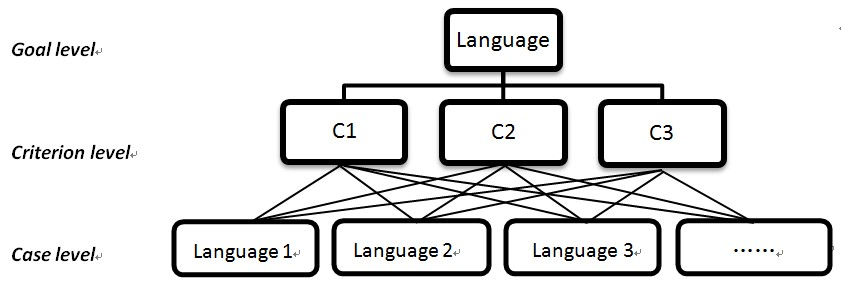
\includegraphics[width=0.8\textwidth]{1}
  \caption{Modeling procedure}
  \label{Modeling procedure}
\end{figure}

According to Analytic Hierarchy Process ($AHP$), we use $a_{ij}$ to represent the influence of $\frac{C_i}{C_j}$ to upper level. After comparing between $C_1$, $C_2$, $C_3$ we can get the Paired Comparison Matrix $A=(a_{ij})_{n\times n}$, and $a_{ij} > 0$, $a_{ij} = \frac{1}{a_{ji}}$

Based on the experience, we can predicate the weight between $C_1$, $C_2$, $C_3$ is $C_1 \colon C_2 = 3 \colon 1 $, $C_2 \colon C_3 = 2 \colon 1 $ and $C_1 \colon C_3 = 2 \colon 1 $, then:
$$A =
 \left[
 \begin{matrix}
   1 & 3 & 4 \\
   \frac{1}{3} & 1 & \frac{1}{2} \\
   \frac{1}{4} & 2 & 1
  \end{matrix}
  \right]
$$

Because $a_{12} \cdot a_{23} \not= a_{13}$, the paired comparison is not completely consistent, and we need to verify the consistency of this matrix.

Firstly, calculating the eigenvalues and corresponding eigenvectors of matrix $A$ by Matlab: $\lambda = 3.1078$, $\vec u = (0.9214, 0.2215, 0.3194)^T$

Then, calculating the Consistency Indicators ($CI$) :
$$CI = \frac{\lambda-n}{n-1} = \frac{3.1078-3}{3-1} = 0.0539$$


And find out Random Consistency Indicators ($RI$) through the table that $RI$=0.58.

\begin{table}[!ht]
  \centering
  \begin{tabular}{ c | c | c | c | c | c | c | c | c | c | c }
    \hline
    $n$ & 2 & 3 & 4 & 5 & 6 & 7 & 8 & 9 & 10 \\ \hline
    $RI$ & 0 & 0.58 & 0.90 & 1.12 & 1.24 & 1.32 & 1.41 & 1.45 & 1.49  \\ \hline
  \end{tabular}
  \caption{The value of RI}
  \label{RI}
\end{table}

Finally, calculating Random Consistency Ratio ($CR$):
$$CR = \frac{CI}{RI} = \frac{0}{0.58} = 0.0929$$

Due to $CR$ < 0.1, we deem matrix A has a satisfied consistency. That is, the eigenvector corresponding to the maximum characteristic root can be used as the weight vector of the comparison factor.

We get the maximum eigenvalue $\lambda = 3$ and corresponding eigenvectors $\vec u = (0.9214, 0.2215, 0.3194)^T$. Then we obtain weight vector $(0.6301, 0.1515, 0.2184)^T$.

Therefore, language development trend coefficient:
$$L = 0.6301C_1 + 0.1515C_2 + 0.2184C_3$$

\subsection{Model B: The number of language speakers in the future prediction model}
Based on the data collected, we decided to use the grey prediction to predict the number of future speakers.

\subsubsection{Analysis}
We believe that there are many reasons for changing the number of speakers in a language. It contains the war, culture communication, international trade and other difficult to standard quantitative indicators, also these indicators have a certain extent of randomness. However, it is clear that these cases effected on past data, in other words, the past data contains all the indicators that affect the number of speakers. Thus, we chose the Grey Model ($GM$) which can predict the data from less past data with a high precision.

\subsubsection{Assumption}
\begin{itemize}
\item There will be no mutation in the short term.
\end{itemize}

\subsubsection{Definition and symbols}
Grey system theory is based on the concept of correlation space and smooth discrete function to define gray derivative and gray differential equation. The dynamic model of differential equation is set up with discrete data column, which is the basic model of the gray system. And the Model is similar and not unique, so this Model is a Grey Model, which is called Grey Model ($GM$), which means Grey Model is made by using discrete random Numbers to become random and the generation number which is significantly weakened and more regular and then establish the model of differential equation form, so as to facilitate the study and description of its change process \cite{5}.

Grey prediction refers to the estimation and prediction of the development and change of system behavior characteristics using $GM$ model.

Simultaneously, it is also possible to estimate the occurrence of abnormal situations of behavior characteristics, as well as the future time distribution of the occurrence of events in a specific time zone and so on.
\begin{table}[!ht]
  \centering
  \begin{tabular}{ c | c }
    \hline
    $x^{(0)}$ & The sample sequences. (Existing data) \\ \hline
    $x^{(1)}$ & Make an Accumulation Generation Operator on $x^{(0)}$  \\ \hline
    $C$ & Posteriori error \\  \hline
  \end{tabular}
  \caption{symbols}
  \label{symbols2}
\end{table}

\subsubsection{Modeling}
Assuming the number of language user over the years is
$$x^{(0)}(1), x^{(0)}(2), ..., x^{(0)}(n)$$

then do an Accumulation Generation Operator ($AGO$), getting a sequence
$$x^{(1)} = (x^{(1)}(1), x^{(1)}(2), ..., x^{(1)}(n)) = (x^{(1)}(1), x^{(1)}(1) + x^{(0)}(2), ..., x^{(1)}(n-1) + x^{(0)}(n))$$

Among that,
$$x^{(1)}(k) = \sum_{i=1}^{k}x^{(0)}(i) \qquad(k = 1, 2, ..., n)$$

Obtaining the Mean sequence that,
$$z^{(0)}(k) = 0.5x^{(1)}(k) + 0.5x^{(1)}(k-1) \qquad(k= 2, 3, ..., n)$$

Then,
$$z^{(1)}=(z^{(1)}(2), z^{(1)}(3), ..., z^{(1)}(n))$$

So we set up the grey differential equation
$$x^{(0)}(k) + az^{(1)}(k) = b, \qquad(k=2, 3, ..., n)$$

The corresponding albino differential equation is
$$\frac{dx^{(1)}}{dt} + ax^{(1)}(t) = b$$

Let,
$$\vec u = (a,b)^T, Y = (x^{(0)}(2),x^{(0)}(3), ..., x^{(0)}(n))^T$$
$$B =
 \left[
 \begin{matrix}
   -z^{(1)}(2) & 1 \\
   -z^{(1)}(3)& 1 \\
   \vdots& \vdots \\
   -z^{(1)}(n)  & 1
  \end{matrix}
  \right]
$$

Based on Least squares method, we led the $J(\vec u)=(Y-B\vec u)^T (Y-B\vec u)$to further getting the minimum value
$$\vec u = (a,b)^{T} = (B^TB)^{(-1)}B^TY$$

Then we solve for the equation that
$$\vec x^{(1)}(k+1) = (x^{(0)}(1) - \frac{b}{a})e^{(-ak)} + \frac{a}{b}, \qquad(k=0, 1, ..., n-1, ...)$$

Then we obtain the predict data
$$\vec x^{(1)}(k+1) = x^{(1)}(k+1) - x^{(1)}(k), \qquad(k=0, 1, ..., n-1, ...)$$


Finally, we utilize After Test Rule to analyze the prediction error and determine the accuracy of the data
$$C = \frac{var(|x^{(1)} - x^{(0)}|)}{var(x^{(0)})}$$
\begin{table}[!ht]
  \centering
  \begin{tabular}{ c | c | c }
    \hline
    Level & posteriori error  C & Error of frequency \\ \hline
    Good & C < 0.35 & P > 0.95 \\ \hline
    Qualified & C < 0.45 & P > 0.80\\  \hline
    Pass &  C < 0.50 & P > 0.70\\  \hline
    Fail &  C < 0.65 & P $\le$ 0.70\\  \hline
  \end{tabular}
  \caption{Accuracy standard of posteriori error \cite{6}}
  \label{error}
\end{table}

\subsection{Model C: Future population of China prediction model}
\subsubsection{Analysis}
China's future population has a huge relationship with China's current birth rate and death rate. Thus, we fitting the difference between birth rate and death rate with the year by the least square method, then solve the differential equation.

\subsubsection{Assumption}
China has had zero net migration in recent years.

\subsubsection{Definition and symbols}

\begin{table}[!ht]
  \centering
  \begin{tabular}{ c | c }
    \hline
    P(x) & The population of China \\ \hline
    x & The year  \\ \hline
  \end{tabular}
  \caption{symbols}
  \label{symbols3}
\end{table}

\subsubsection{Modeling}
We found the following data from the world bank.

\begin{table}[!ht]
  \resizebox{\textwidth}{!}{
  \centering
  \begin{tabular}{ c | c | c | c | c | c | c | c | c | c }
    \hline
     & 1972 & 1977 & 1982 & 1987 & 1992 & 1997 & 2002 & 2007 & 2012 \\ \hline
     Mortality (per thousand people) & 7.61 & 6.87 & 6.6 & 6.72 & 6.64 & 6.51 & 6.41 & 6.93 & 7.15  \\ \hline
     Birth rate (per thousand people) & 29.77 & 18.93 & 22.28 & 23.33 & 18.27 & 16.57 & 12.86 & 12.1 & 12.1  \\ \hline
     Difference value & 22.16 & 12.06 & 15.68 & 16.61 & 11.63 & 10.06 & 6.45 & 5.17 & 4.95  \\ \hline
  \end{tabular}
  }
  \caption{1972-2012 Mortality and Birth rate in China}
  \label{Mortality and Birth rate}
\end{table}

Then, we use Matlab to fitting the difference value with years by the least square method,and get the result:

$$Linear\ model\ Poly_1: f(x) = p_1 \times x + p_2$$
$$Cofficients(with\ 95\%\  confidence\ bound)$$
$$p_1 = -0.3827(-0.5431, -0.2224)$$
$$p_2 = 774.1(454.6, 1093)$$

Integrating both sides of this equation
$$\int f(x)dx = \int -0.3827x + 774.1dx$$

Then,
$$P(x) = -0.19135x^2 + 774.1x + C$$

The real population in 1972 is 862030000, plug this number in above function and figure out the C equal to 861247593.62.

 Therefore,
 $$P(x) = -0.19135x^2 + 774.1x + 861247593.62$$



\section{Application}
We will apply the model mentioned above to solve the practical problem. The process will be divided into two steps: Data processing and Problem solving.

\subsection{Data processing}
\subsubsection{Predict: the number of users $C_1$}
Firstly, we utilize Model B to predict the number of language users in 50 years.
We selected 14 languages with the largest number of people in the previous years, and obtained the previous year's data by searching.
\begin{table}[!ht]
  \centering
  \begin{tabular}{ c | c | c | c | c | c }
      \hline
       & 2017 \cite{7} & 2014 \cite{8} & 2011 \cite{9} & 2009 \cite{10} & 2005 \cite{11} \\ \hline
      Mandarin Chinese& 1090 & 1197 & 1284 & 1213 & 1051 \\ \hline
      English & 983 & 335 & 372 & 328 & 510 \\  \hline
      Hindustani & 544 & 260 & 260 & 182 & 490 \\  \hline
      Spanish & 527 & 414 & 437 & 329 & 420 \\  \hline
      Arabic & 422 & 237 & 295 & 221 & 230 \\  \hline
      Malay & 281 &  & 60.8 & 39.1 &  \\  \hline
      Russian & 267 & 167 & 154 & 144 & 255 \\  \hline
      Bengali & 261 & 193 & 242 & 181 & 215 \\  \hline
      Portuguess & 229 & 203 & 219 & 178 & 213 \\  \hline
      French & 229 & 75 & 76.1 & 67.8 & 130 \\  \hline
      Japanese & 129 & 122 & 128 & 122 & 127 \\  \hline
      German & 129 & 78.2 & 76.8 & 90.3 & 229 \\  \hline
      Korean & 77 & 77.2 & 77.2 & 66.3 & 71 \\  \hline
      Panjabi & 148 &  &  & 62.6 & 88 \\  \hline
  \end{tabular}
  \caption{Total number of language users(million)}
  \label{Total number of language users(million)}
\end{table}

Subsequently, we plotted the data into a line chart, and simply observed the trend of the number of language users.
\begin{figure}[!hb]
  \centering
  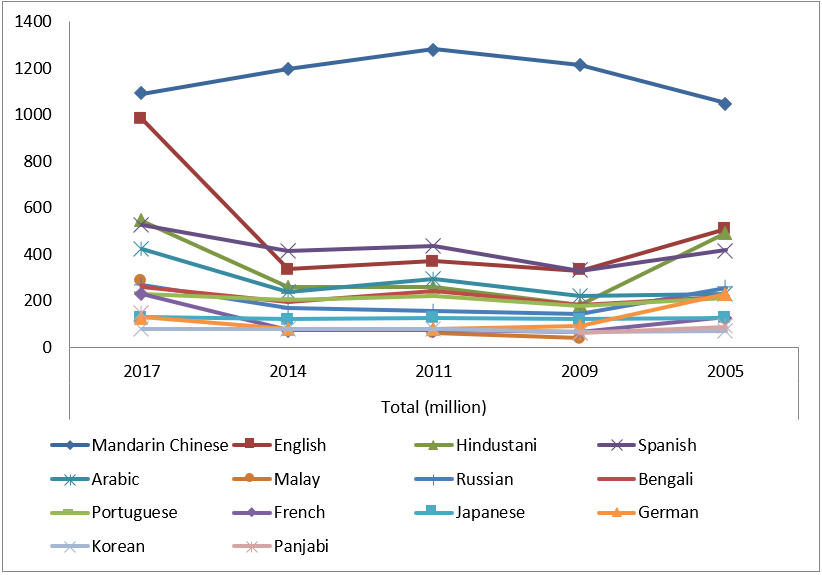
\includegraphics[width=0.8\textwidth]{3}
  \caption{Results}
  \label{Res}
\end{figure}

We plug the data into model b, take the state as a unit, and calculated the result by Matlab. Then we sorted the data in descending order according to the data size of “After 50 years”, and got the following table.
\begin{table}[!ht]
  \centering
  \begin{tabular}{ c | c | c | c }
    \hline
    Language & After 30 years & After 50 years & C \\ \hline
    English & 1190.2410 & 1922.2897 & 0.3246\\  \hline
    Mandarin Chinese & 1089.3346 & 1049.7645 & 0.2687 \\ \hline
    Hindustani & 525.9848 & 707.5967 & 0.1670 \\  \hline
    Spanish & 588.6219 & 672.9143 & 0.2526 \\  \hline
    Arabic & 475.1541 & 586.7825 & 0.3402 \\  \hline
    French & 265.8385 & 459.6159 & 0.3219\\  \hline
    Malay & 350.2279 & 440.1033 & 0.3057 \\  \hline
    Russian & 309.2814 & 388.8702 & 0.2172  \\  \hline
    Portuguese & 243.1803 & 259.5467 & 0.3482  \\  \hline
    Bengali & 271.4378 & 248.6587 & 0.3494 \\  \hline
    German & 175.9098 & 203.3289 & 0.1253  \\  \hline
    Japanese & 127.5109 & 135.3985 & 0.3444  \\  \hline
    Panjabi & 127.3669 & 110.0944 & 0.3239  \\  \hline
    Korean & 82.6025 & 86.2441 & 0.3343  \\  \hline
    \end{tabular}
  \caption{the number of language speakers After 30 or 50 years for each languages}
  \label{the number of language speakers After 30 or 50 years for each languages}
\end{table}

The posterior difference ratio of each prediction data is less than 0.35, so we believe that the prediction accuracy is relatively high.

Therefore, we can conclude that compared to the total number of language users in 2017 the member of top 10 in next 50 years do not have any change. However, the order has a dramatic change. For instance, English will become the most spoken language.

\subsubsection{Language difficulty rating $C_2$}
We find out the following official report published by Government Accountability Office ($GAO$) as a reference criterion for rating.

Note: In order to facilitate the view, we marked the selected language.
\begin{figure}[!ht]
  \centering
  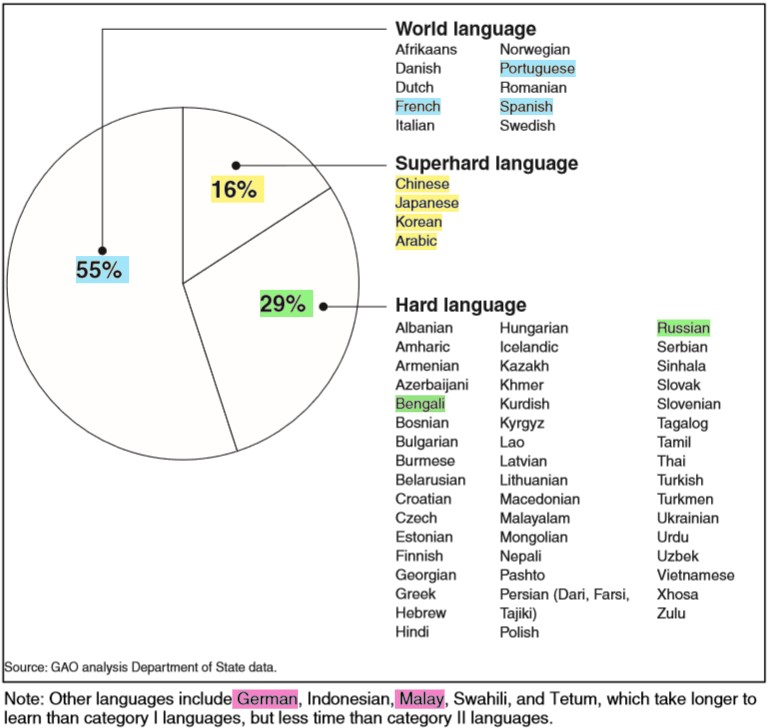
\includegraphics[width=0.6\textwidth]{4}
  \caption{Language difficulty rating standard \cite{12}}
  \label{Language difficulty rating standard}
\end{figure}

According to the figure, we select the proportion as the score to evaluate the difficulty of language. Based on the precondition of problem that all of the employee have master English, we set the score as 100.

(Note: as the difficulty increasing, the score decreasing)
\begin{table}[!ht]
  \resizebox{\textwidth}{!}{
  \centering
  \begin{tabular}{ c | c | c | c | c | c | c | c }
    \hline
    Language & Mandarin Chinese & English & Hindustani & Spanish & Arabic & Malay & Russian \\ \hline
    Score & 16 & 100 & 29 & 55 & 16 & 35.5 & 29 \\ \hline
    Language & Bengali & Portuguese & French & Japanese & German & Korean & Panjabi \\  \hline
    Score & 29 & 55 & 55 & 16 & 35.5 & 16 & 35.5 \\  \hline
  \end{tabular}
  }
  \caption{Language difficulty rating scale}
  \label{Language difficulty rating scale}
\end{table}

\subsubsection{Language family $C_3$}
Following is the integration information from Ethnologue \cite{1}.
\begin{table}[!ht]
  \centering
  \begin{tabular}{ c | c  }
    \hline

    Mandarin Chinese & Sino-Tibaten, Sinitic \\ \hline
    English & Indo-European, Germanic\\  \hline
    Hindustani &Indo-European, Indo-Aryan  \\  \hline
    Spanish & Indo-European, Romance \\  \hline
    Arabic & Afro-Asiatic, Semitic \\  \hline
    Malay & Austronesian, Malayo-Polynesian  \\  \hline
    Russian & Indo-European, Slavic  \\  \hline
    Bengali & Indo-European, Indo-Aryan  \\  \hline
    Portuguese & Indo-European, Romance  \\  \hline
    French & Indo-European, Romance  \\  \hline
    Japanese & Japonic  \\  \hline
    German & Indo-European, Germanic \\  \hline
    Korean & Koreanic  \\  \hline
    Panjabi & Indo-European, Indo-Aryan  \\  \hline
  \end{tabular}
  \caption{Language Family}
  \label{Language Family}
\end{table}

According to the analysis of the previous analysis (the language of similar languages family is more acceptable), it is reasonable to assume that the 14 languages are graded according to the language family.

(Note: Assuming that English is the native language, the following data can be obtained based on the similarity ratio of language family.)
\begin{table}[!ht]
  \centering
  \begin{tabular}{ c | c | c | c | c | c | c | c }
    \hline
    Language & Mandarin Chinese & English & Hindustani & Spanish & Arabic & Malay & Russian \\ \hline
    Percentage($\%$) & 0 & 100 & 50 & 50 & 0 & 0 & 50 \\ \hline
    Language & Bengali & Portuguese & French & Japanese & German & Korean & Panjabi \\  \hline
    Percentage($\%$) & 50 & 50 & 50 & 0 & 100 & 0 & 50 \\  \hline
  \end{tabular}
  \caption{Language difficulty rating scale}
  \label{Language difficulty rating scale}
\end{table}


\subsection{Problem solving}
In order to provide the best working language choice for the client company, we plug the data obtained above into Model A, and obtained the corresponding scores of each language, and sorted the scores from large to small, and reached the following table.
\begin{table}[!ht]
  \centering
  \begin{tabular}{ c | c  }
    \hline
    \ & language & Score \\ \hline
    English & 765.3393\\  \hline
    Mandarin Chinese & 688.8137\\ \hline
    Spanish & 379.3324 \\  \hline
    Hindustani & 335.9257  \\  \hline
    Arabic & 301.8186 \\  \hline
    Malay & 226.0568  \\  \hline
    Russian & 199.3809  \\  \hline
    French & 175.9465  \\  \hline
    Bengali & 175.5357  \\  \hline
    Portuguese & 161.6696  \\  \hline
    German & 116.4374 \\  \hline
    Panjabi & 85.74133  \\  \hline
    Japanese & 82.76862  \\  \hline
    Korean & 54.47184  \\  \hline
  \end{tabular}
  \caption{The order of prediction result }
  \label{The order of prediction result }
\end{table}

We use model C to predict the population of China over the next 50 years.
$$P(x) = -0.19135x^2+774.1x + 861247593.62 $$
$$P(2068) = -0.19135 \times 2068^2 + 774.1 \times 2068 + 861247593.62 = 862030100.42$$

As can be seen from the comparison, the change of population has no effect on the geographical distribution of language users.

\begin{figure}[!ht]
  \centering
  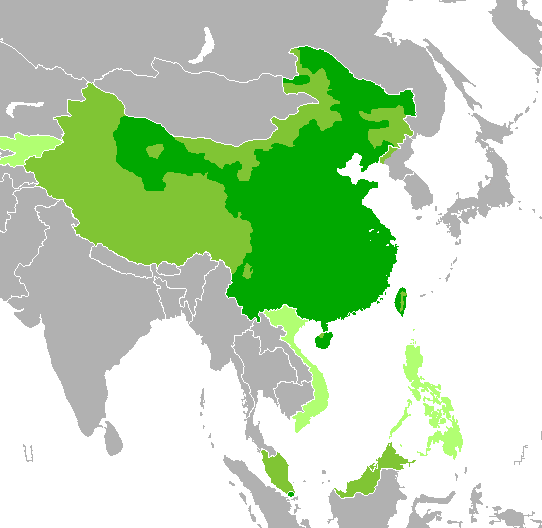
\includegraphics[width=0.6\textwidth]{5}
  \caption{the geographical distribution of language users}
  \label{the geographical distribution of language users}
\end{figure}

Therefore, when choosing an office location for the client company, our main concern is the local economy.

The Gross Domestic Product ($GDP$) is the total value of the various sectors of the national economy that a country or region added in a certain period of time [14], so we choose $GDP$ as the basis for judging the economic level of each country.

In order to reduce the error, we accumulate the $GDP$ index from 1960 to 2016 and rank the country according to it.

Following table shows the data of top 14 countries.
\begin{table}[!ht]
  \centering
  \begin{tabular}{ c | c  }
    \hline
     & Country & Accumulation of $GDP$(1960-2016)($\$$) \\ \hline
    America & $38.6083 \times 10^{13}$\\  \hline
    Japan & $15.1888 \times 10^{13}$\\ \hline
    China & $10.2059 \times 10^{13}$\\  \hline
    German & $8.94624 \times 10^{13}$ \\  \hline
    France & $6.58257 \times 10^{13}$ \\  \hline
    United Kingdom & $6.48233 \times 10^{13}$  \\  \hline
    Italy & $5.28358 \times 10^{13}$  \\  \hline
    Brazil & $3.61641 \times 10^{13}$  \\  \hline
    Canada & $3.51382 \times 10^{13}$  \\  \hline
    Spain & $3.00586 \times 10^{13}$  \\  \hline
    India & $2.90331 \times 10^{13}$ \\  \hline
    Russian & $2.51573 \times 10^{13}$  \\  \hline
    Mexico & $2.37087 \times 10^{13}$  \\  \hline
    Korea & $2.29995 \times 10^{13}$  \\  \hline
  \end{tabular}
  \caption{The order of prediction result }
  \label{The order of prediction result }
\end{table}

We combine the official language used by the countries in figure 9 with figure 8 to take the intersection. (Note: set language as major premise, and the company already has offices in New York and Shanghai.)

Following are our final result.
\begin{figure}[!ht]
  \centering
  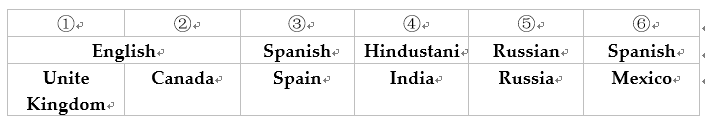
\includegraphics[width=0.8\textwidth]{6}
  \caption{ final result}
  \label{Resul}
\end{figure}



\section{Weakness}
\subsection{Model A}
\begin{itemize}
\item The setting of indicators and weights is subjective and lacks the theoretical support of professional systems.
\item Restricted by the selected index, the influence of other aspects cannot be taken into account, lead to resulting in a certain deviation from the true weight vector.
\end{itemize}
\subsection{Model B}
\begin{itemize}
\item The long-term value cannot be accurately predicted.Because the sample size is small, the prediction data can only reach an ideal accuracy in the short term. With the increase of time, the predicted data will deviate significantly.
\item  Selected data -- the total number of people using a certain language is not necessarily accurate due to different statistical time, which leads to certain errors in the predicted data.
\end{itemize}
\subsection{Model C}
\begin{itemize}
\item Factors that affect the population in addition to birth and death are not considered.
\end{itemize}

\begin{thebibliography}{99}
\bibitem{1} Wikipedia (2018), Ethnology
https://en.wikipedia.org/wiki/Ethnologue
\bibitem{2}Ethnology (2017)
https://www.ethnologue.com/
\bibitem{3}Fan. J. J (2006), Language vitality and language endangered assessment, Modern Foreign Languages (Quarterly)
http://www.ixueshu.com/document/473743860c879c6b.html
\bibitem{4}Lu. X. Y (2002), The positive role of first language in second language acquisition, Foreign Language World No.4 2002(General Serial No.90)
http://www.wanfangdata.com.cn/details/detail.do?type=perioid=QK200200558766
\bibitem{5} Si. S. K (2007), Mathematical modeling algorithms and procedures, Naval aviation engineering college, Chapter 25 Grey system theory and application, p551-555
\bibitem{6}Ning. X. X, Liu. S. F. (2009), Management forecasting and decision-making methods [M]. Beijing: science press, p113-145.
\bibitem{7}Wikipedia (2017), List of languages by total number of speakers
https://en.wikipedia.org/wiki/Listoflanguagesbytotalnumberofspeakers
\bibitem{8} Ethnology (2014)
http://www.ethnologue.com/17/statistics/
\bibitem{9} Ethnology (2011), Summary by language size
https://www.ethnologue.com/statistics/size
\bibitem{10} M. Paul Lewis (2009), Statistic summary, Ethnology
http://www.ethnologue.com/16/ethnodocs/distribution/size/
\bibitem{11} Vistawide (2005), Top 30 Languages by Number of Native Speakers
 http://www.vistawide.com/languages/top30languages.htm
\bibitem{12} United States Government Accountability Office (2006), GAO-06-894, Staffing and Foreign Language Shortfalls Persist Despite Initiatives to Address Gaps, State’s Foreign Language Requirements, p10
https://www.gao.gov/assets/260/251024.pdf
\bibitem{13} The World Bank Group (2018), GDP (current US$\$$)
https://data.worldbank.org/indicator/NY.GDP.MKTP.CD
\end{thebibliography}
\end{document}

%%
%% This work consists of these files mcmthesis.dtx,
%%                                   figures/ and
%%                                   code/,
%% and the derived files             mcmthesis.cls,
%%                                   mcmthesis-demo.tex,
%%                                   README,
%%                                   LICENSE,
%%                                   mcmthesis.pdf and
%%                                   mcmthesis-demo.pdf.
%%
%% End of file `mcmthesis-demo.tex'.
